\documentclass[journal]{IEEEtran}
%\documentclass[conference]{IEEEtran}
\hyphenation{op-tical net-works semi-conduc-tor}
\usepackage{graphicx}
\graphicspath{{./images/}}

\begin{document}
\title{Low Cost Real-time Room Occupancy Indicating System}
\author{Chirag~Shah, Srijal~Poojari and Priya~Deshpande
\\
Department of Electronics Engineering, Sardar Patel Institute of Technology, Mumbai.}



\maketitle
\begin{abstract}
The objective of this action research based project was to tackle a problem faced by corporate environments. The typical corporate office consists of several meeting rooms with employees requiring frequent access to these meeting rooms, but lack of real-time knowledge of its availability leads to inconvenient hassle. The proposed solution consists of a network of motion detection sensors (namely, the PIR sensor) spread out across all meeting rooms, updating the room occupancy status in real-time to a central base-station, a desktop computer, from which it can be relayed to the employees using a web server or a smartphone application.

Each sensor node is designed to be Low Cost, Wireless and Low Power for seamless integration and to avoid frequent battery replacement.
\end{abstract}


\section{Introduction}
\IEEEPARstart{I}{n} a typical corporate environment there exists multiple conference/meeting rooms.
The site that we studied was at Fractal Analytics, Goregaon. The office has around 400 employees: 250 employees on 7th floor, 150 employees on 3rd floor. 7th floor has 10 meeting rooms and 3rd floor has 5 meeting rooms. Anyone can book any meeting room for any time (if the room is available) using a mobile app. This is an open office - hence if anyone wants to have a discussion then they need to go to a meeting room. Hence meeting rooms are always in demand.


The problem was that anyone could book a meeting room and then not use it. Or if someone wanted to have a meeting without prebooking the meeting room the he/she would have to go from room to room to check the availability of the rooms. The would create a lot of unnecessary hassle and would lead to unoptitmal utilization of the workspace.


To solve these problem we envisioned a solution which would involve placing sensors in every meeting room to monitor the occupancy of the room. This sensor will then relay the real time occupancy information of the room to a central device which will keep track of the occupancy status of all the meeting rooms. This data can then be showed on a web/mobile interface to check the real time occupancy status of the meeting room or the data can be integrated with the the mobile app to automatically book or cancel the meetings as per the occupancy of the rooms.


\section{System Design}
\subsection{Prototype breadboards}
For testing purposes, we have designed the prototype of the circuit on breadboards which included the microcontroller, radio module and an OLED display

\begin{figure}[ht]
	\centering
	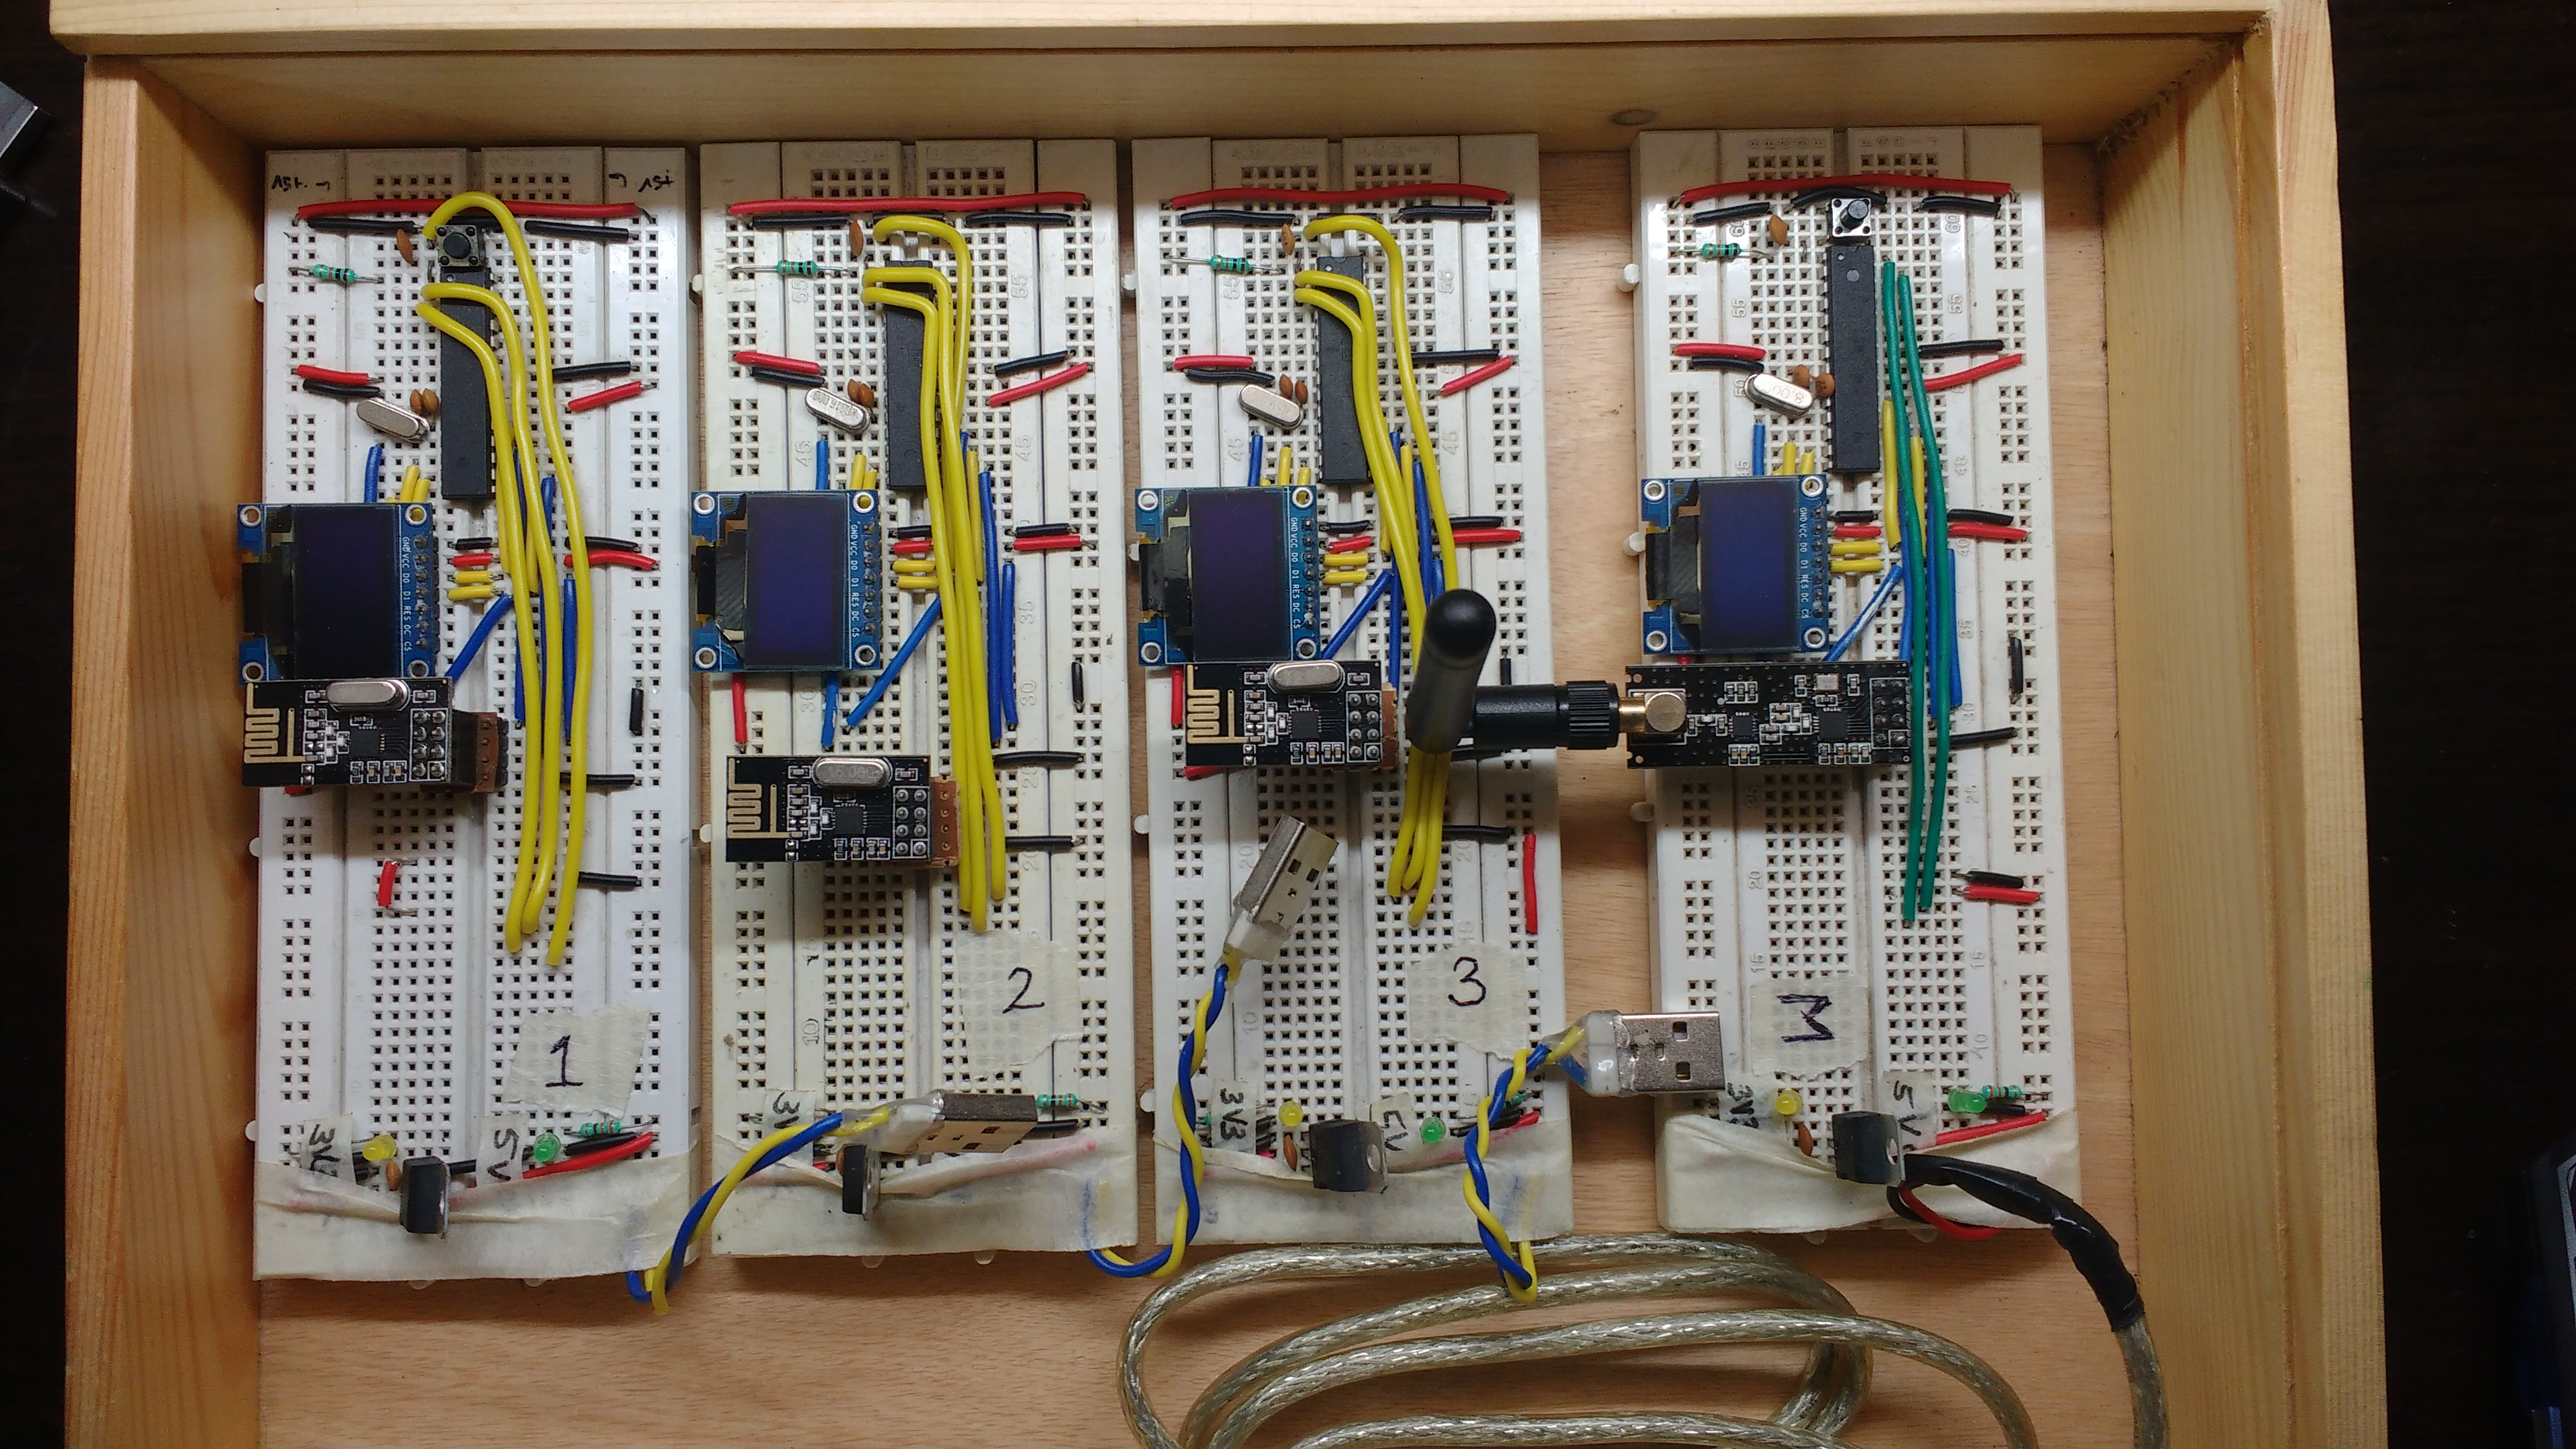
\includegraphics[scale=0.06]{all_breadboards.jpg}
	\caption{The 4 breadboard prototypes}
	\label{fig_breadboard}
\end{figure}

\subsection{Low Power Design}
We desired a battery life of 3-12 months before the battery needs to be replaced. Hence to reduce the active and standby current of our circuit we took the following steps.

\begin{itemize}	
	\item When the device is not transmitting the microcontroller and the radio module go into a deep sleep state. The current consumption reduces to \textbf{80$\mu$A}. 
	\begin{itemize}
		\item \textbf{50$\mu$A} is used by the PIR sensor when motion is not detected. (150$\mu$A when motion is detected)
		\item \textbf{20$\mu$A} is the quiescent current of the voltage regulator
		\item \textbf{9$\mu$A} is the current consumption of the ATmega $\mu$C
		\item \textbf{1$\mu$A} is taken by the nrf module in the \textbf{deep sleep} state
	\end{itemize}
	
	\item We have taken various measures to reduce the power consumption of the ATmega $\mu$C.
	\begin{enumerate}
		\item Put the processor to power down mode. This is the most power efficient sleep mode. This disconnects the clock from the CPU, flash memory, IO ports, ADC. It also disconnects the external crystal oscillator and the timer oscillator. BOD is also disabled. The only way to wake up the $\mu$C is by WDT or by external interrupts.
		\item Arrange to wake the processor from sleep only when needed based on watchdog timer overflow and interrupt by the PIR sensor
		\item Run the processor at a lower frequency (8Mhz)
		\item Run the processor at a lower voltage (3V) (This will also reduce the number of batteries to be used as the supply voltage reduces)
		\item Turn off unneeded internal modules in software (eg. SPI, I2C, Serial, ADC). This will reduce the power consumption $\mu$C is awake. They are disabled by default in the sleep state
		\item Turn off brownout detection
		\item Turn off the Analog-to-Digital converter (ADC). This will reduce the power consumption $\mu$C is awake. It is disabled by default in the sleep state
		\item Set not required pins to output
	\end{enumerate} 
\end{itemize}

\subsection{PCBs}
Later we created PCBs using Autodesk Eagle and had it manufactured so that each node is of a small form-factor and is reliable. For this SMD components are used wherever possible. Ports for a Real Time Clock (RTC) is provided for future use in improving the low power capabilities.

\begin{figure}[ht]
	\centering
	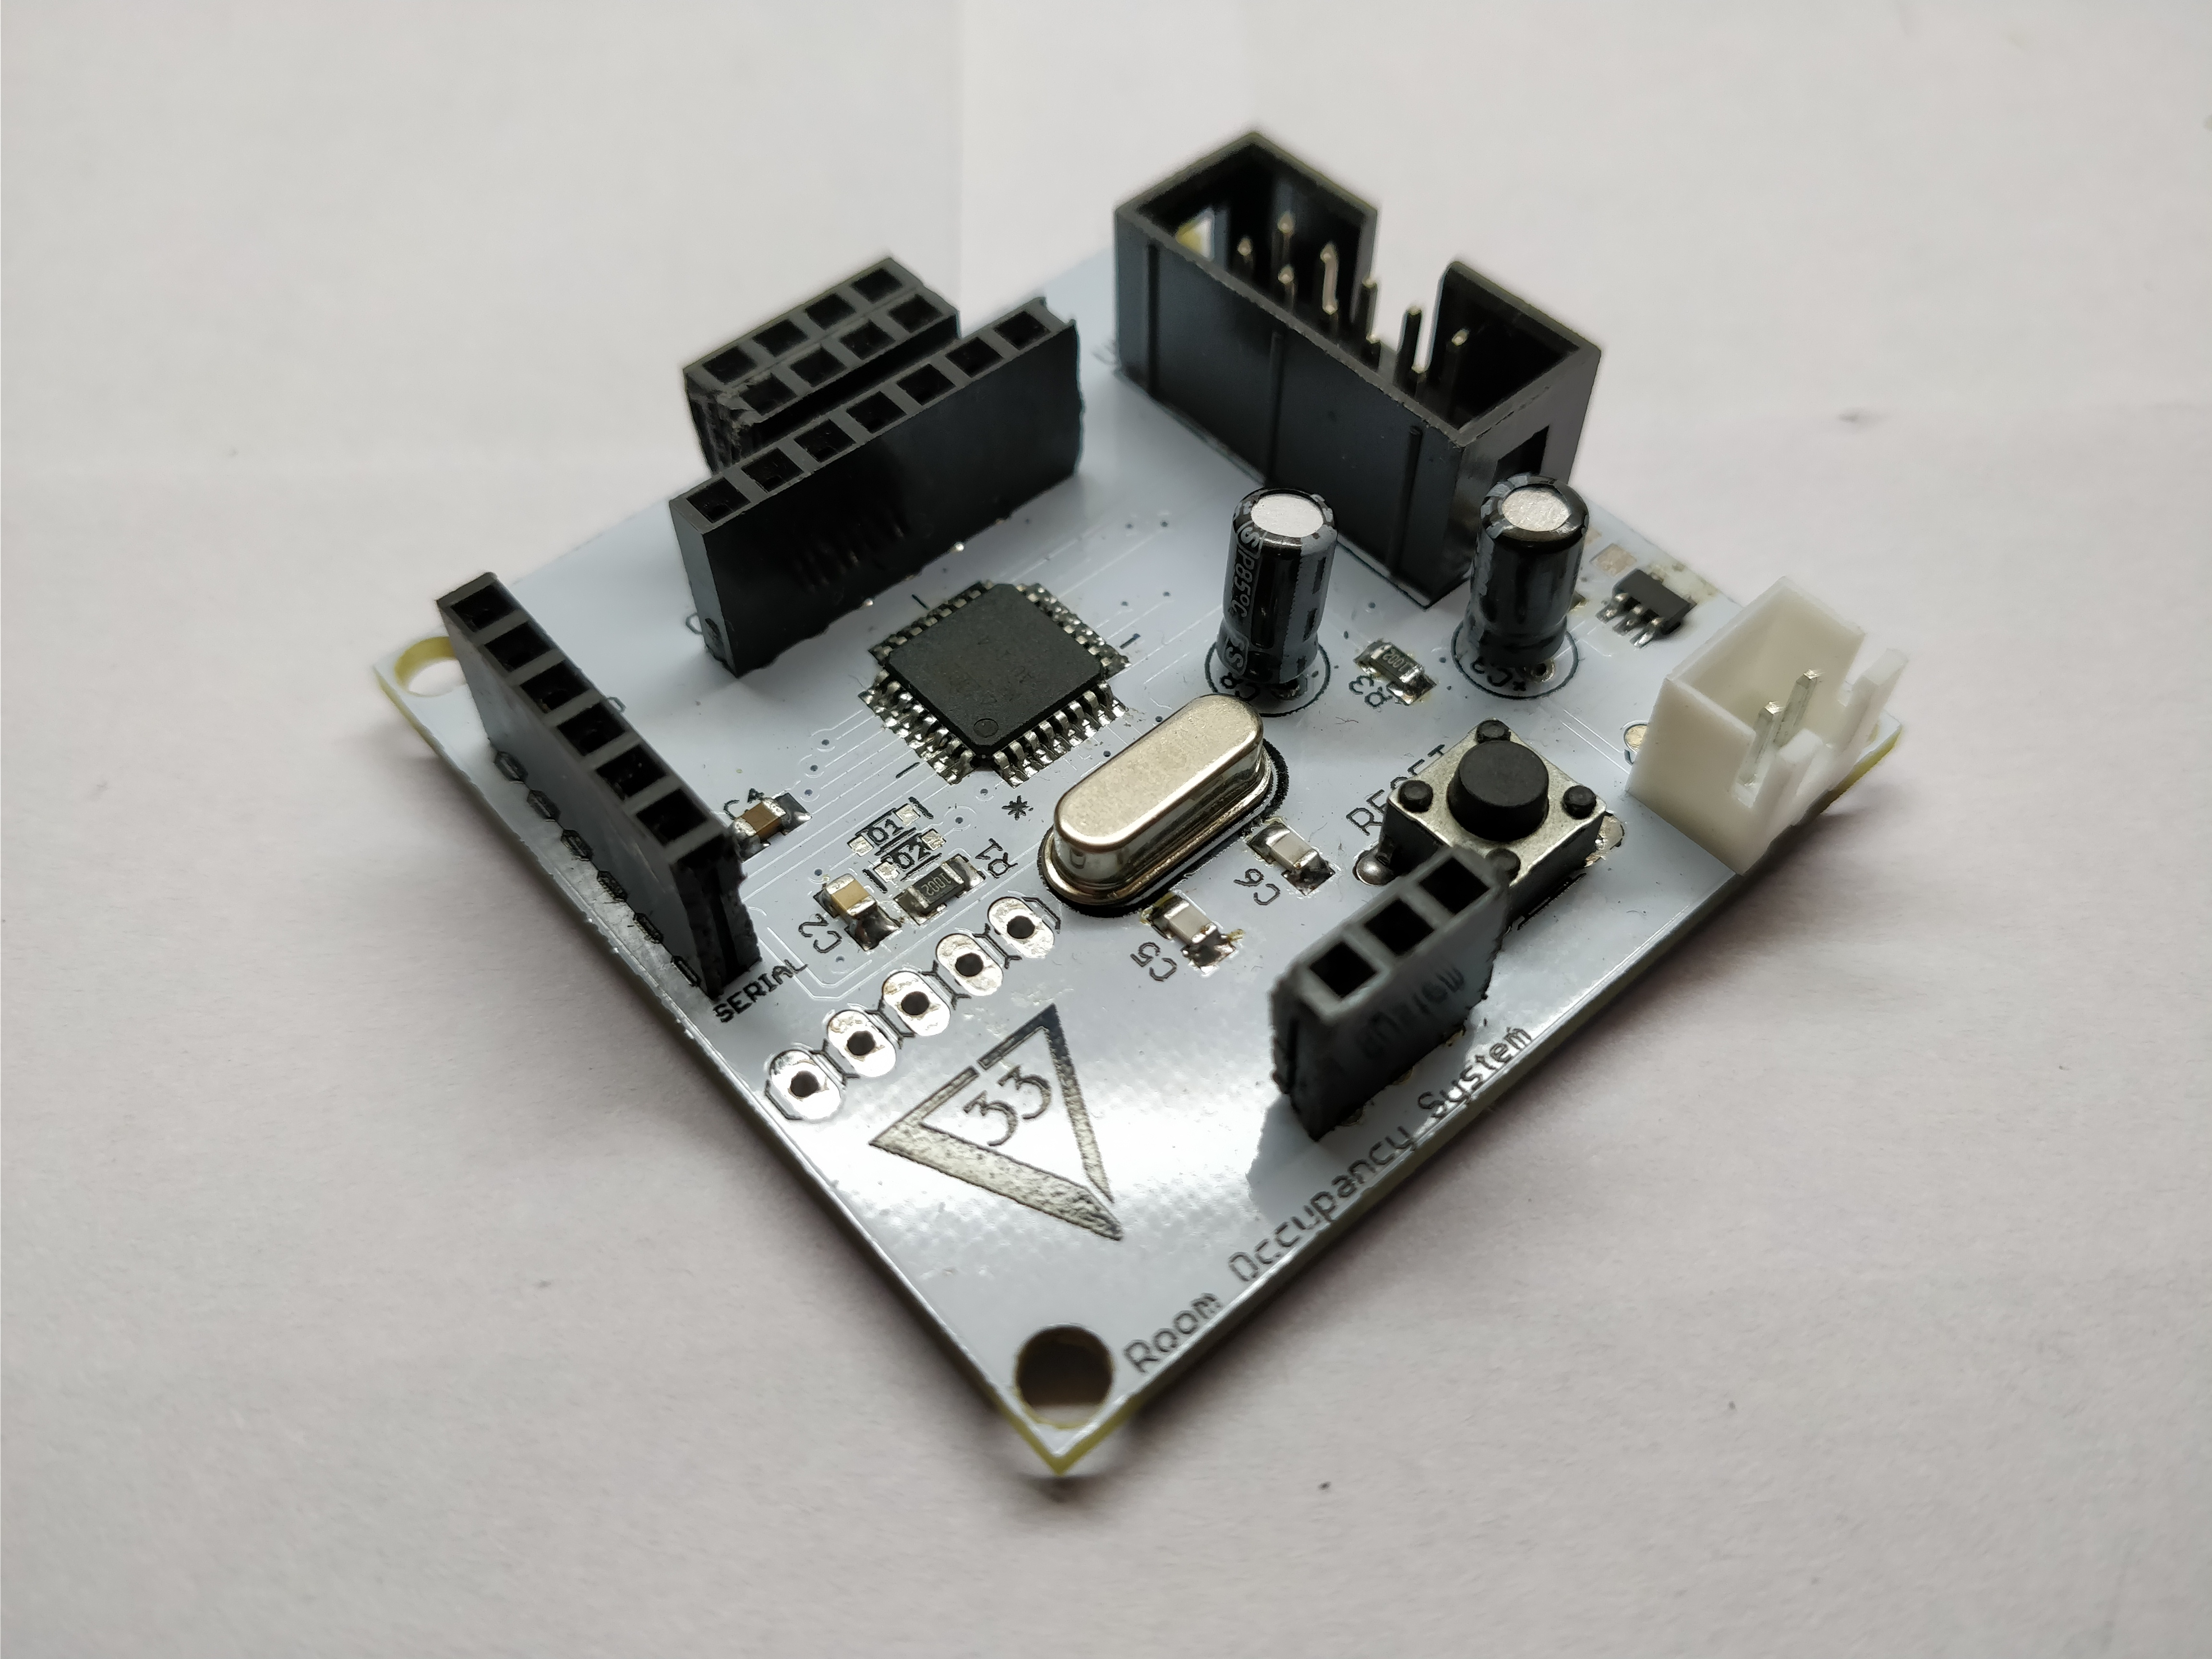
\includegraphics[scale=0.05]{1__30_.jpg}
	\caption{The PCB created}
	\label{fig_pcb}
\end{figure}

\subsection{Enclosure}
The enclosure was designed on Autodesk Fusion 360 and 3D printed for a professional look.

\begin{figure}[ht]
	\centering
	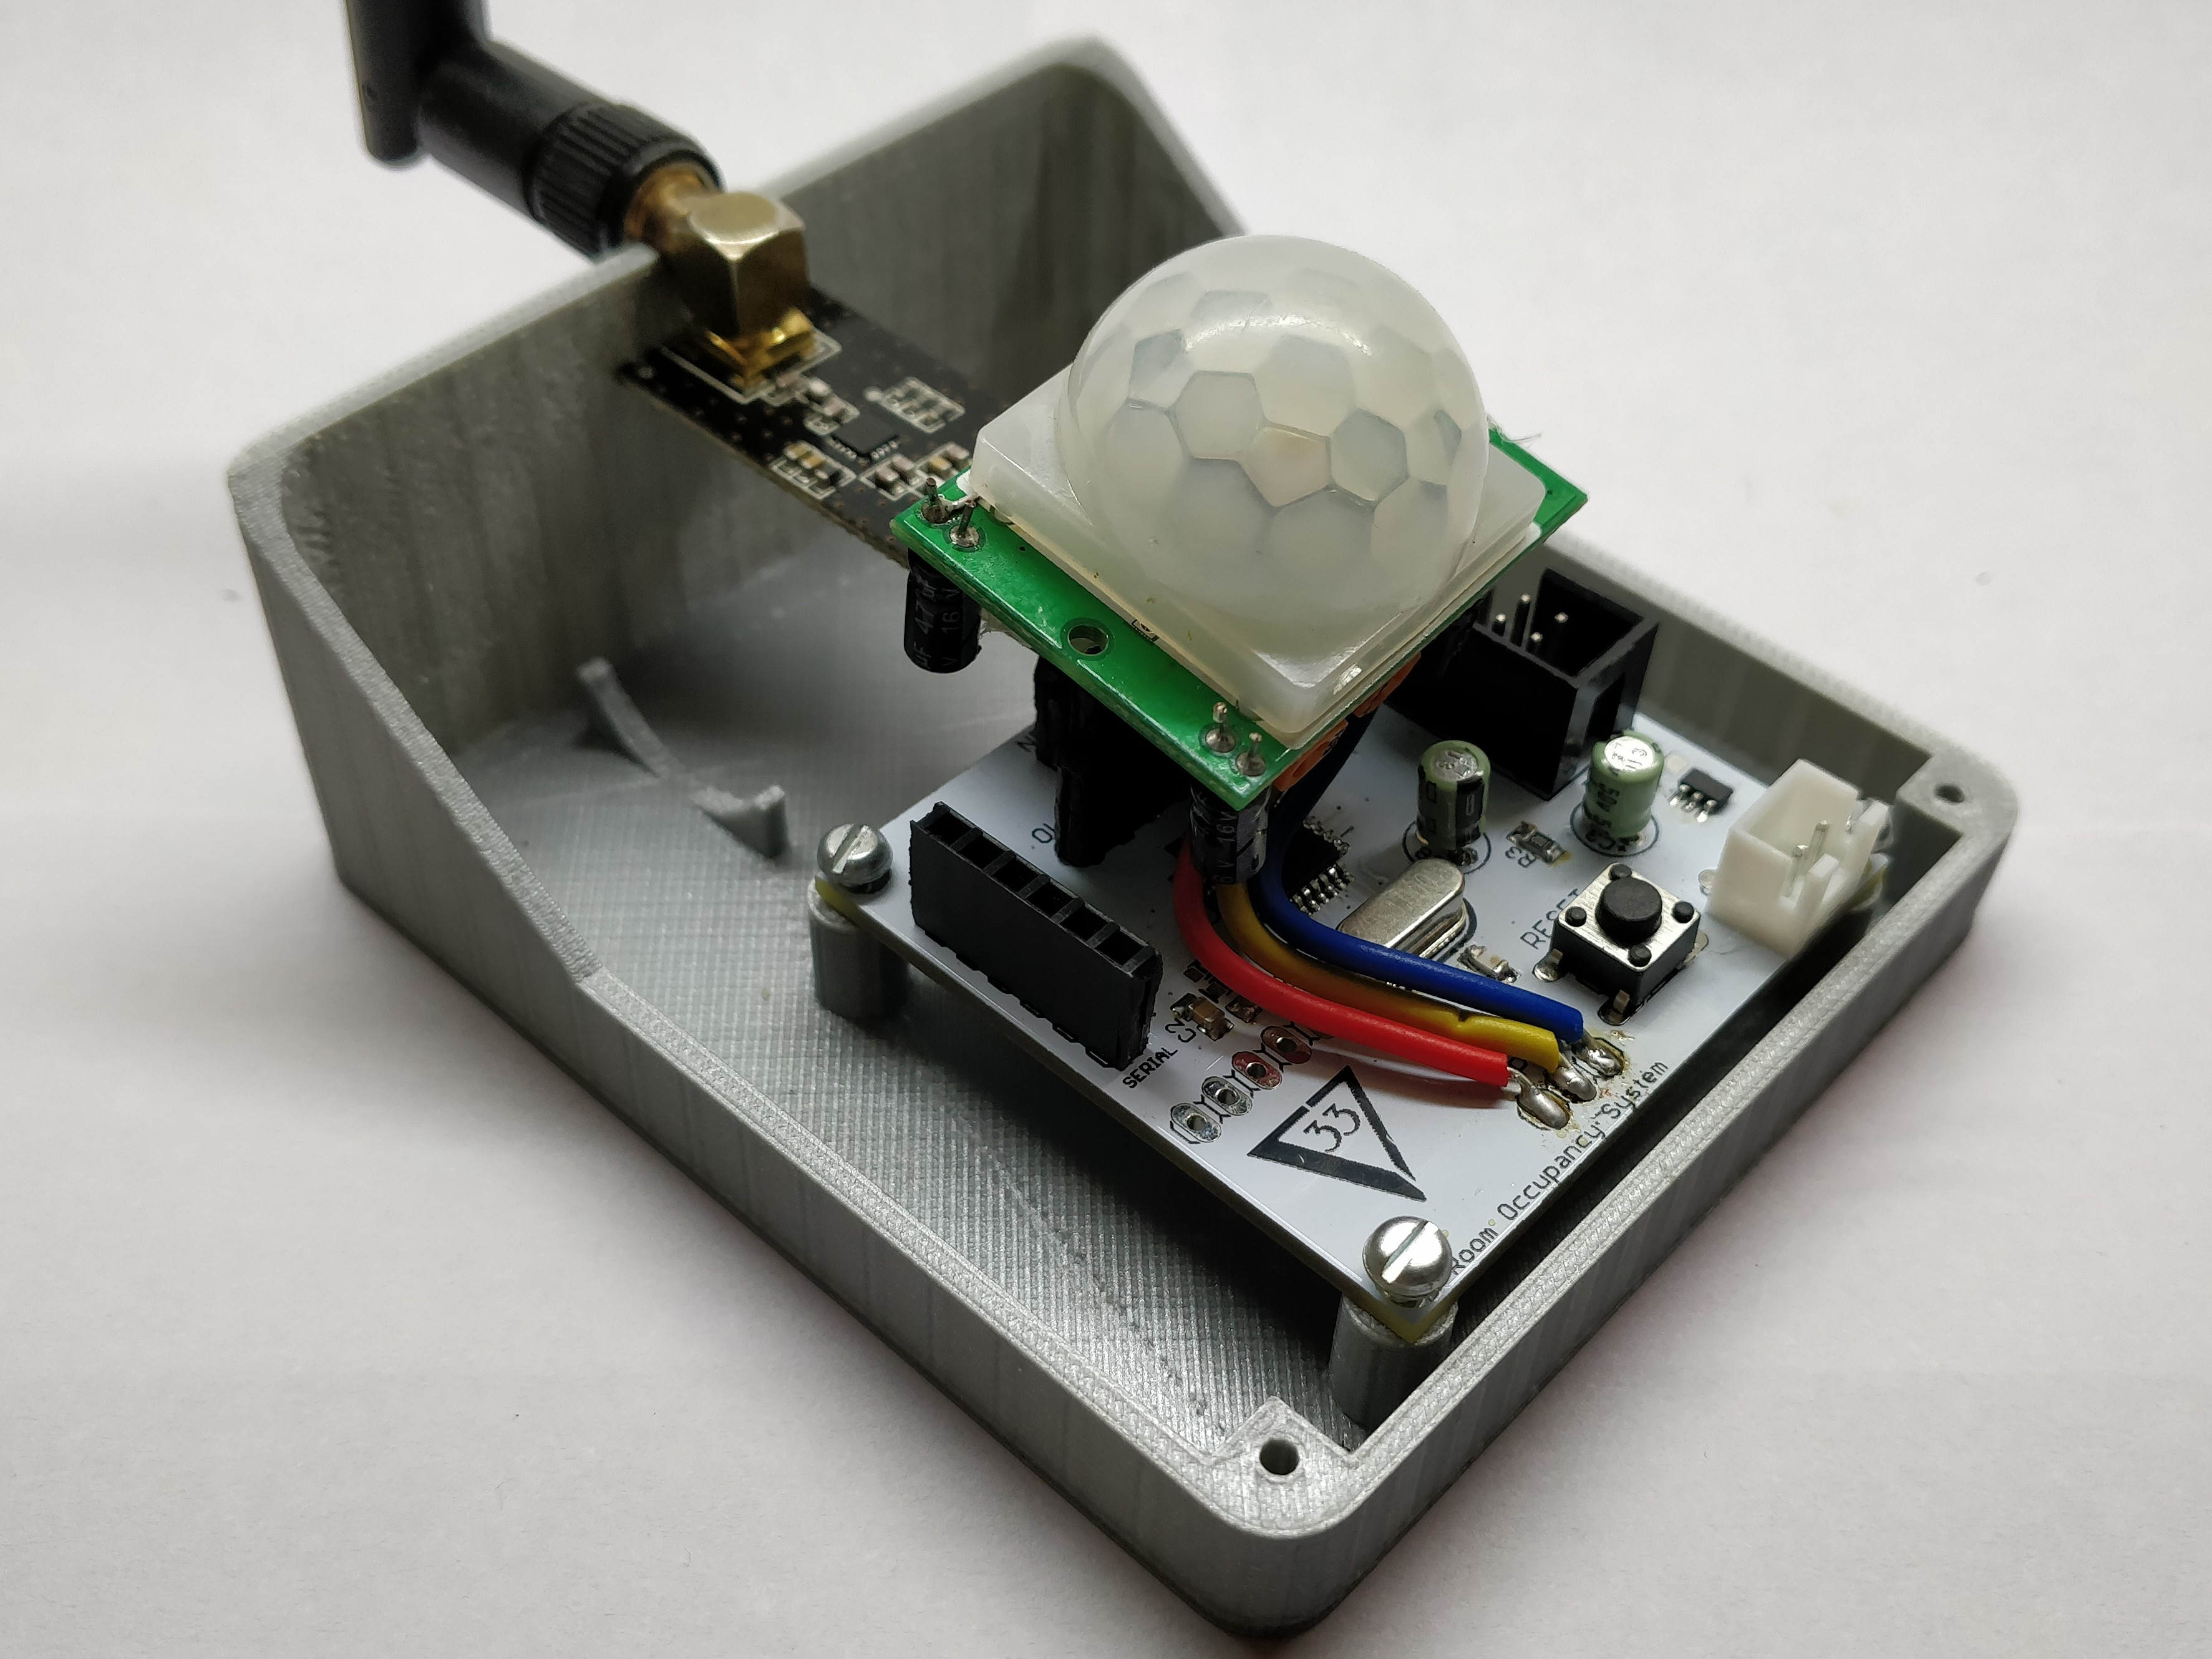
\includegraphics[scale=0.05]{AssemPCB2.jpg}
	\caption{The printed enclosure with PCB}
	\label{fig_enclosure}
\end{figure}


\section{Results}
All the end nodes stay in a deep sleep state. They wake up only when a change of state in the PIR sensor is detected or when the WDT overflows. 

When motion is detected the device wakes up from its deep sleep state using interrupts and then transmits the required information and goes back to its deep sleep state. 
The devices also periodically wake up and send the state when the WDT overflows. This is so that if a device fails the master can sense that the device hasn't transmitted anything recently and then that device can be marked offline by the user.

The routers are always awake and listening so that they can route information between the devices and the master whenever required. They can be battery powered or can be powered using a mains adapter.

The current of the end nodes is 18mA when transmitting but it is only 80$\mu$A when it is in standby mode. This will significantly improve the battery life of the devices.

All the devices are configured in a tree network configuration to increase the range of the network. Each NRF24 Module can support upto 6 slave devices simultaneously, so the network has to be designed appropriately while setting it up in any real environment.

\begin{figure}[ht]
\centering
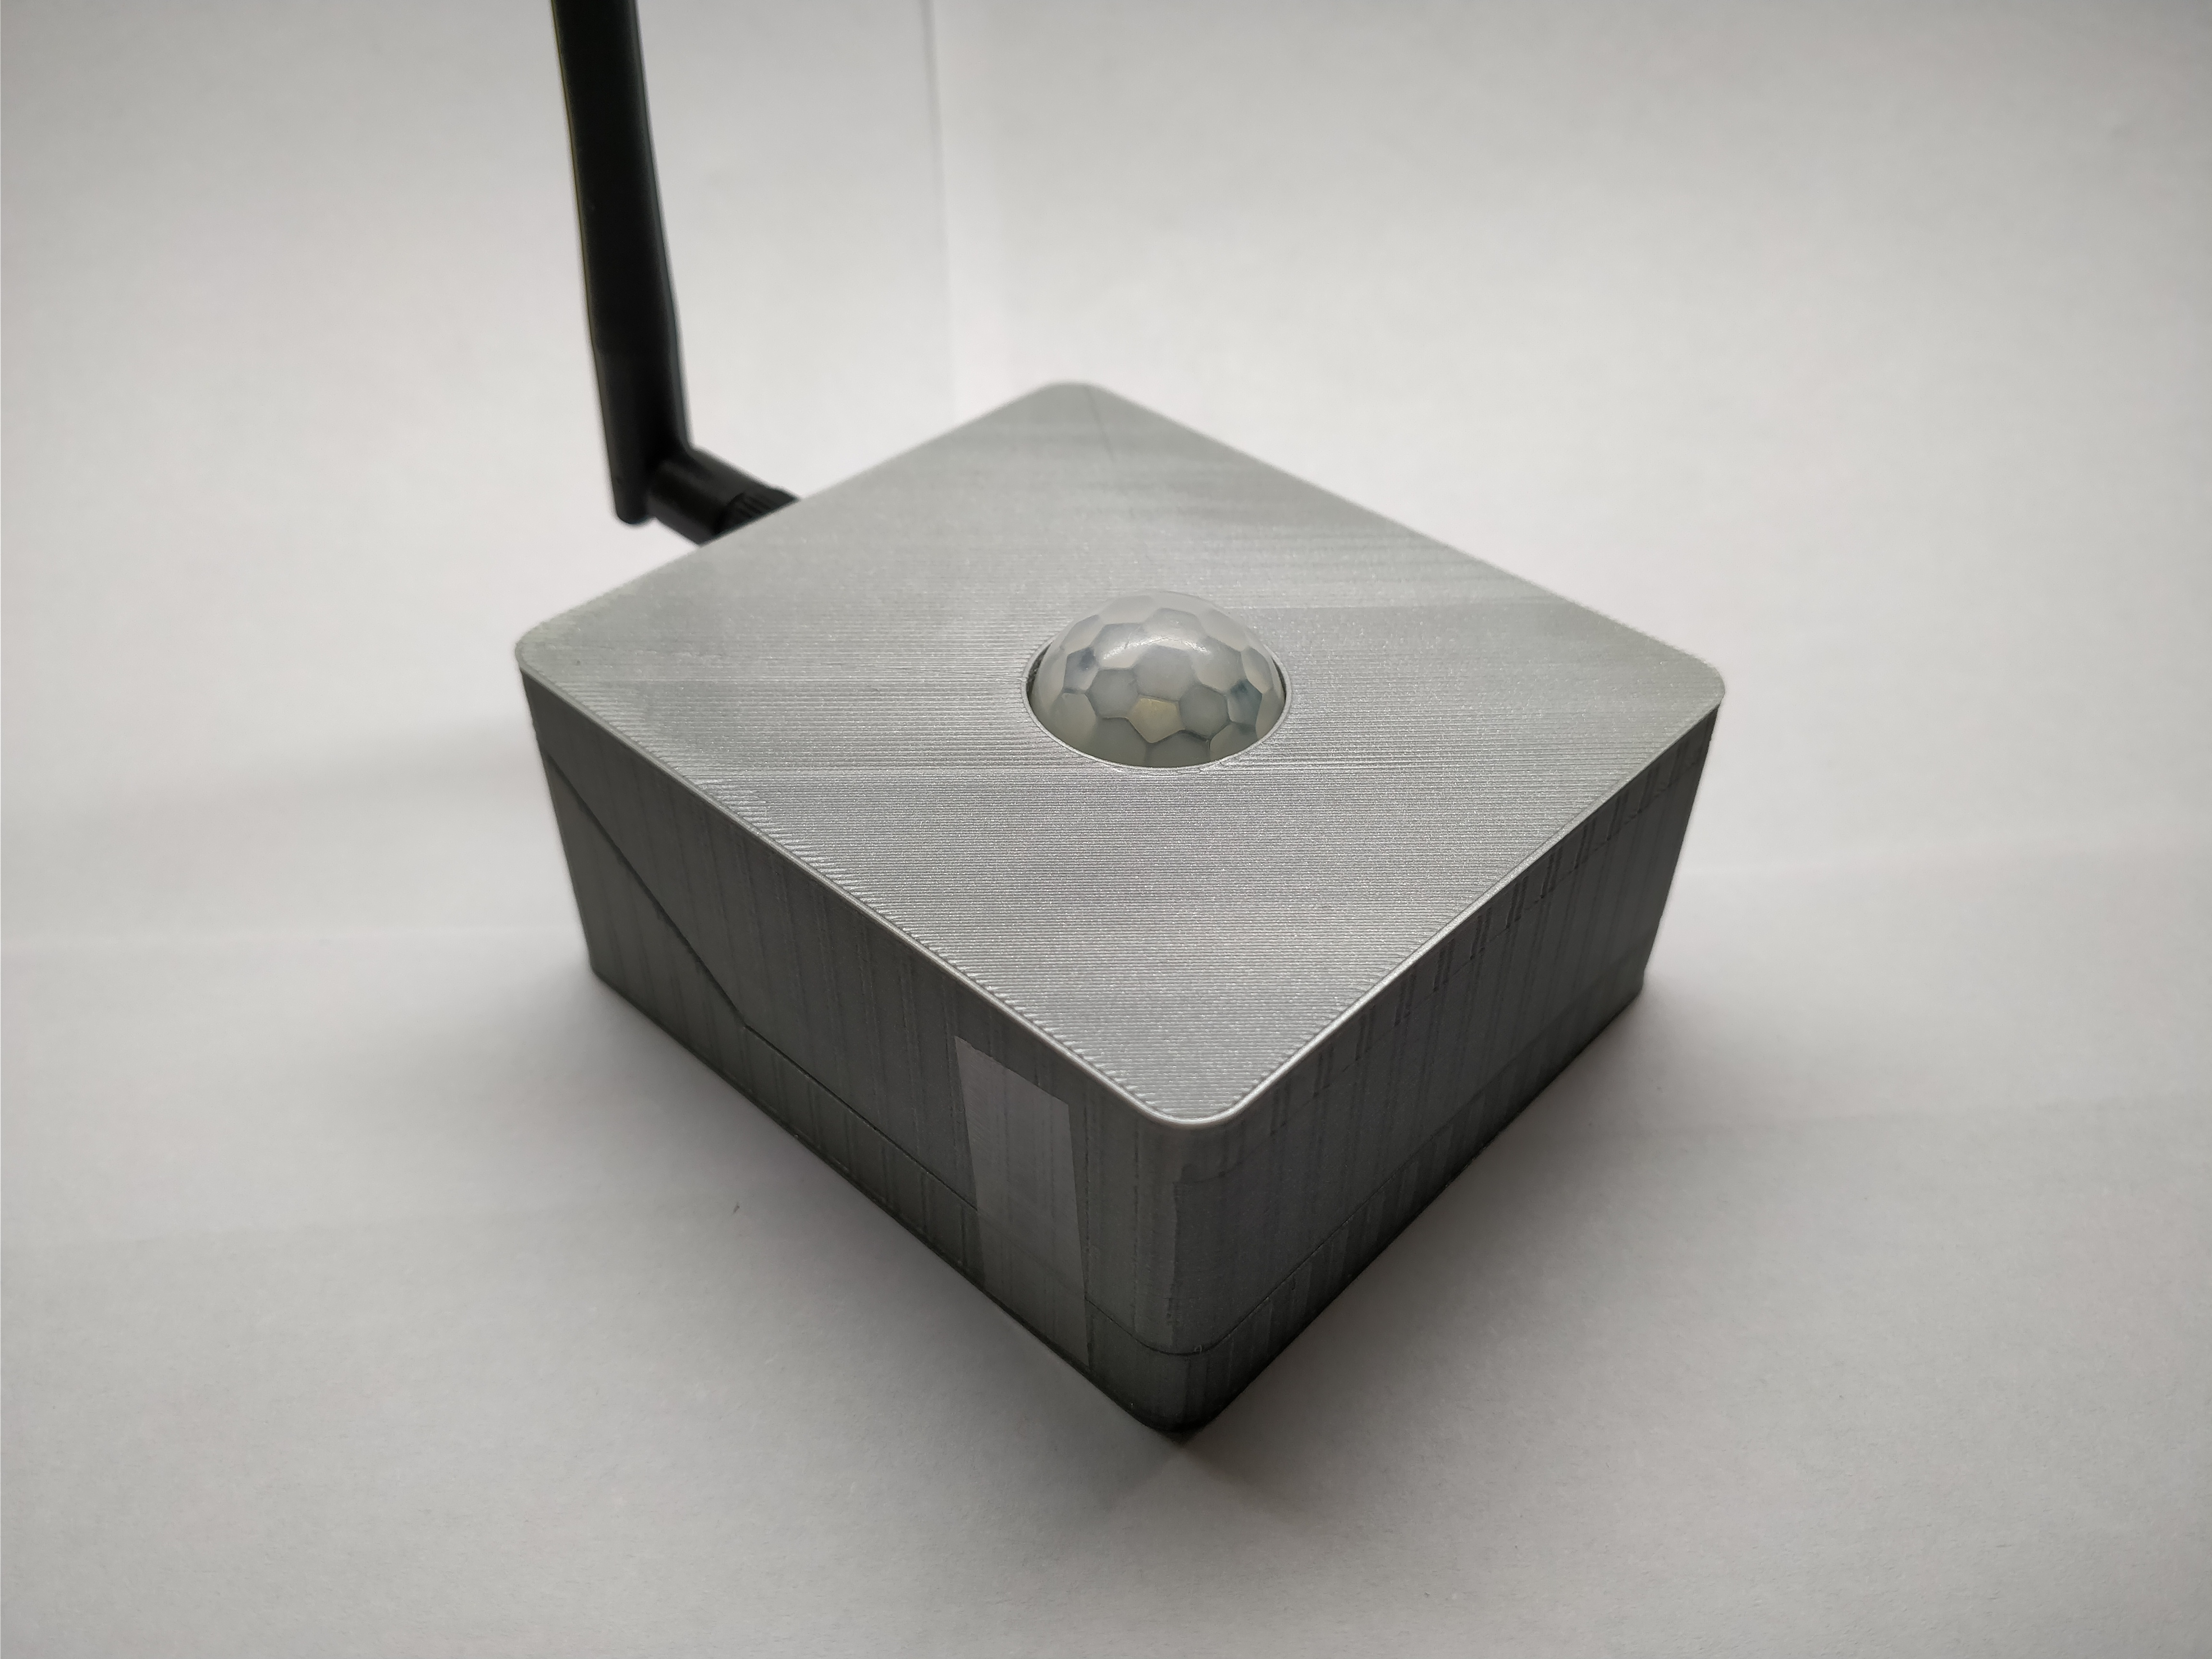
\includegraphics[scale=.05]{FinalProduct.jpg}
\caption{Final Assembled Device}
\label{fig_final}
\end{figure}

Real time occupancy status can be seen on any web browser. The colours indicate state of each node. Green and Red indicate that the node is ON and actively sensing, and their sensor state is represented. The time since the current state has occured is also shown. Greyed out nodes are not active and are either switched OFF or their connection is broken. 
 
\begin{figure}[ht]
	\centering
	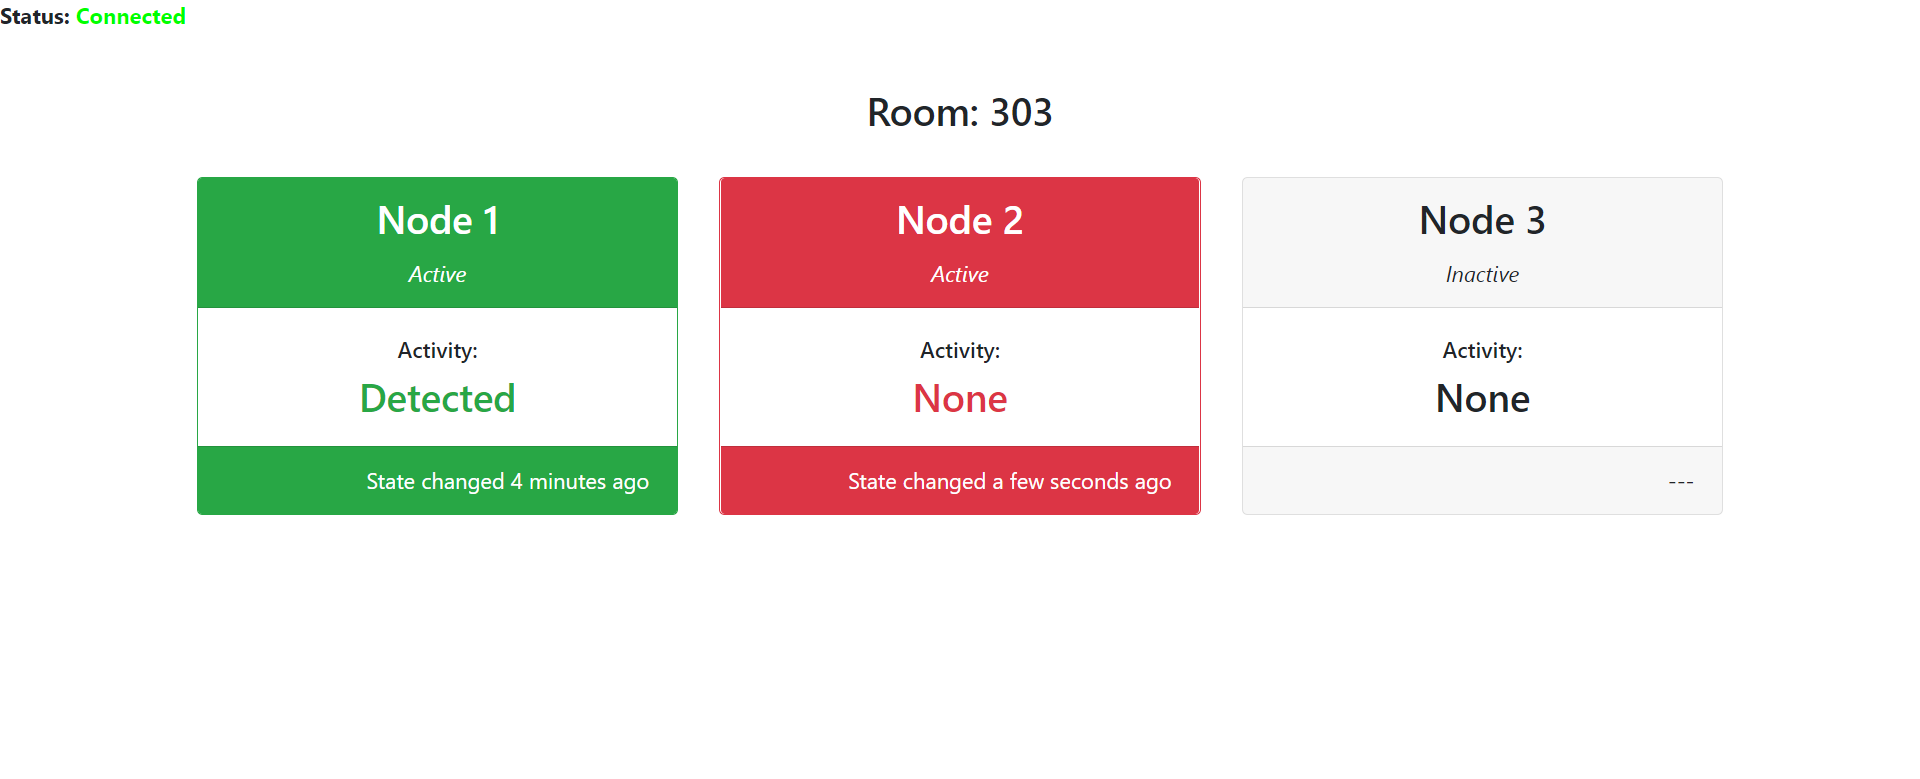
\includegraphics[scale=.2]{Website1.PNG}
	\caption{Web GUI}
	\label{fig_gui}
\end{figure}

\section{Conclusion}
We were able to create a wireless tree network of low powered battery operated devices which which would sense the occupancy of each room and then relay the occupancy status to a central master device. The device then relayed the real time occupancy status to a local server. A web browser (client) can then dynamically, using websockets, view the status of each node in real-time.

The cost per device (~900 INR) is much less than the current available commercial alternatives such as Workscape\cite{workscape} and Occupeye\cite{occupeye}, which typically are priced at 15\textdollar \hspace{1pt} per device per month, as stated earlier. Hence the goal of making a low cost device has been achieved.

The software can be greatly improved further to make the system robust and easily scalable, but the system at its current state is a lays a strong foundation for future development.

There are also a few hardware changes that could be made such as rearranging the components on the PCB for a smaller form-factor and utilizing the RTC port for such as alarm interrupt for sending heartbeat packets, and get more power savings by a complete shutdown after office hours, holidays etc.


\section*{Acknowledgments}

We would like to take this opportunity to thank Aashish Nehete for his immense help in creating and designing the web-based GUI for this project. We are also grateful to Prof. Kaiser Katchi for his help in 3D printing the project enclosure.
Special thanks to our institute, Sardar Patel Institute of Technology, for providing us with 3D printing services and a platform for us to showcase our project.


% Can use something like this to put references on a page
% by themselves when using endfloat and the captionsoff option.
\ifCLASSOPTIONcaptionsoff
  \newpage
\fi



% trigger a \newpage just before the given reference
% number - used to balance the columns on the last page
% adjust value as needed - may need to be readjusted if
% the document is modified later
%\IEEEtriggeratref{8}
% The "triggered" command can be changed if desired:
%\IEEEtriggercmd{\enlargethispage{-5in}}

% references section

% can use a bibliography generated by BibTeX as a .bbl file
% BibTeX documentation can be easily obtained at:
% http://mirror.ctan.org/biblio/bibtex/contrib/doc/
% The IEEEtran BibTeX style support page is at:
% http://www.michaelshell.org/tex/ieeetran/bibtex/
%\bibliographystyle{IEEEtran}
% argument is your BibTeX string definitions and bibliography database(s)
%\bibliography{IEEEabrv,../bib/paper}
%
% <OR> manually copy in the resultant .bbl file
% set second argument of \begin to the number of references
% (used to reserve space for the reference number labels box)
\begin{thebibliography}{1}

\bibitem{sparkfun}
~Sparkfun.com, `nRF24L01+ Transceiver Hookup Guide,' [Online].
Available:https://learn.sparkfun.com/tutorials/nrf24l01-transceiver-hookup-guide 
[Accessed: 10-Feb-2018]

\bibitem{geekstips}
~geekstips.com, `Internet of Things Project, Communication between ESP8266 modules,' [Online]. Available: https://www.geekstips.com/two-esp8266-communication-talk-each-other/ [Accessed: 18-Feb-2018] 

\bibitem{grabcad}
~GrabCAD, `Free cloud-based collaboration solutionto view and share CAD files,' [Online].
Available:https://grabcad.com/ [Accessed: 20-Mar-2018]

\bibitem{pcbway}
~PCBWay `PCB Manufacturing service'  [Online].
Available:https://pcbway.com/ [Accessed: 12-Mar-2018]

\bibitem{occupeye}
~Occupeye `OccupEye workspace utilisation sensors'  [Online].
Available:https://occupeye.com/ [Accessed: 11-Feb-2018]

\bibitem{workscape}
~Workscape `Workscape smart sensors'  [Online].
Available:https://workscape.io/ [Accessed: 11-Feb-2018]

\bibitem{github}
~ROIS on Github, `Room Occupancy Indicating Network,'  [Online].
Available:https://github.com/Nabla33/Room\_Occupancy\_Indicating\_Network [Accessed: 18-May-2018]


\end{thebibliography}

\end{document}


